\documentclass[a4j]{jarticle}

\usepackage{additional}

\setlength{\voffset}{-1truein}
% \setlength{\hoffset}{-1truein}

\setlength{\topmargin}{28truemm}
\setlength{\headheight}{0truemm}
\setlength{\headsep}{0truemm}

\newcommand{\vtr}[1]{\mbox{\boldmath $#1$}}

\makeatletter
	\renewcommand{\theequation}{%
  \thesection.\arabic{equation}}
  \@addtoreset{equation}{section}

\makeatother

\title{隠れマルコフモデル \\ Hidden Markov Model}
\author{山下 滉}
\date{2017/04/21}

\begin{document}

\maketitle

\section{マルコフ連鎖}
「コイントスして,表なら左へ一歩,裏なら右へ一歩」を延々と繰り返すという最も基本的な確率過程のことを\textbf{ランダムウォーク(酔歩)}という.
左右の確率を変えたり前後左右へ動くようにしたりと,バリエーションはいろいろ考えられるが,ここでは単純に一次元で左右等確率の設定とする.
形式的に書くと,$+1$か$-1$かが半々の確率で出るi.i.d\footnote{独立同一分布(independent and indentically distributed; i.i.d)}な確率変数たち$Z_{1}, Z_{2}, Z_{3},...$を使って,
\begin{equation}
X_{0}=0, \quad X_{t} = X_{t-1} + Z_{t} \ (t=1,2,...) \label{eq:ranwark}
\end{equation}
と表される$X_{t}$のことである\cite{probability_statistics_for_programming}.

ランダムウォークの場合,
\begin{equation}
P(X_{t+1} = x_{t+1} | X_{t} = x_{t},X_{t-1} = x_{t-1}, ... , X_{0} = x_{0}) = P(X_{t+1}=x_{t+1}|X_{t} = x_{t}) \label{eq:markov}
\end{equation}
が成り立つ.
つまり,未来の状態は今の状態だけから定まり,過去の履歴(どこからどんな経路をたどって今の状態にたどりついたか)には無関係であった.
現在の状態が一時点前の状態に依存して確率的に決まるような特性を\textbf{マルコフ性(Markov property)}という.
そしてこのような確率過程を\textbf{マルコフ過程(Markov process)}という.
その中でも特に,$X_{t}$がとり得る値が有限とおりなものを\textbf{マルコフ連鎖(Markov chain)}と呼ぶ.

マルコフモデルは複数の状態を持ち,ある状態から別の状態(元の状態も含む)へ一定の確率で遷移する.
この確率を\textbf{遷移確率(transition probability)}という.
また,現在の状態に依存した一定の確率で特定の\textbf{出力記号(output symbol)}を出力する.
この確率を\textbf{出力確率(output probability)}という\cite{probability_statistics_for_programming}.

\begin{figure}[H]
	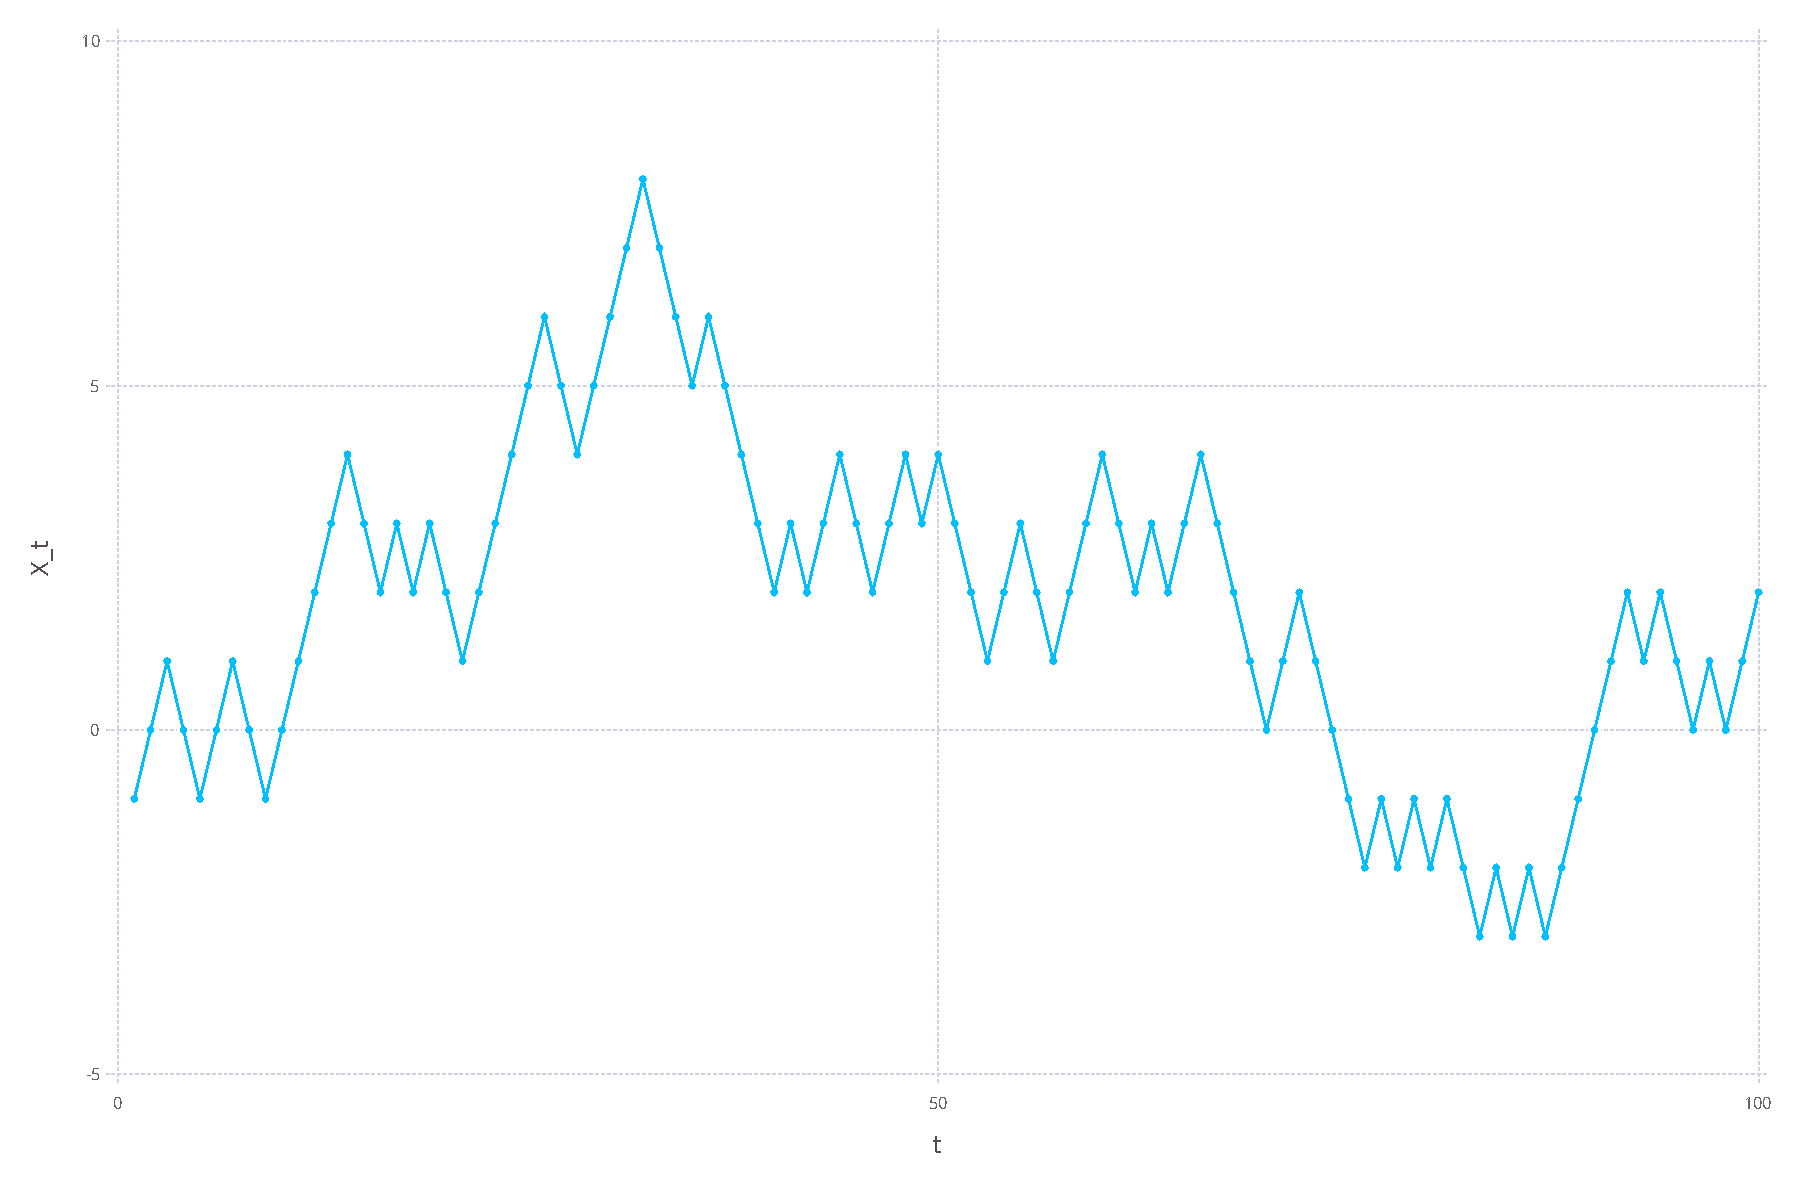
\includegraphics[width=1.5\hsize,angle=-90, bb=0 0 864 576]{./fig/hidden_markov_model/random_walk.pdf}
	\caption{ランダムウォークの例}
	\label{}
\end{figure}

\newpage

\section{マルコフモデル}
例として,3種類のサイコロ$\omega_{1}$,$\omega_{2}$,$\omega_{3}$を投げて出た目を観測する場合を考える.
ここではサイコロの目として奇数と偶数の2種類を考える.

遷移確率行列$\bm{A}$,出力確率行列$\bm{B}$が以下のように与えられたとする.

\begin{equation}
\bm{A} = \hspace{1zw}
\bordermatrix{
	& \omega_{1} & \omega_{2} & \omega_{3} \cr
	\omega_{1} & 0.1 & 0.4 & 0.5 \cr
	\omega_{2} & 0.2 & 0.1 & 0.7 \cr
	\omega_{3} & 0.3 & 0.1 & 0.6 \cr
}
\end{equation}

\begin{equation}
\bm{B} = \hspace{1zw}
\bordermatrix{
	& 奇数 & 偶数  \cr
	\omega_{1} & 0.8 & 0.2  \cr
	\omega_{2} & 0.6 & 0.4  \cr
	\omega_{3} & 0.3 & 0.7  \cr
}
\end{equation}

行列$\bm{A}$により,遷移確率$a_{ij}$を反映した状態遷移系列が得られる.
状態遷移の様子を図\ref{fig:markov:markovmodel}(\subref{fig:markov:markovmodel1})に示す.
行列$\bm{B}$は,サイコロ$\omega_{1}$,$\omega_{2}$,$\omega_{3}$を投げて奇数の目が出る確率がそれぞれ$0.8,  0.6,  0.3$,偶数の目が出る確率がそれぞれ$0.2,  0.4,  0.7$であることを示している.

時刻$t$における状態を$s_{t}$,出力記号を$x_{t}$として,マルコフモデルをグラフィカルモデルで表したものを図\ref{fig:markov:markovmodel}(\subref{fig:markov:markovmodel2})に示す.
マルコフモデルでは状態系列と出力系列の両方を観測することができる.この観測値から$\bm{A},\bm{B}$などのパラメータを推定するのがマルコフモデルの問題である.
状態系列が与えられていることから,マルコフモデルは教師あり学習であるといえる.

\begin{figure}[htb]
	\centering
	\begin{minipage}[t]{.49\hsize}
		\centering
		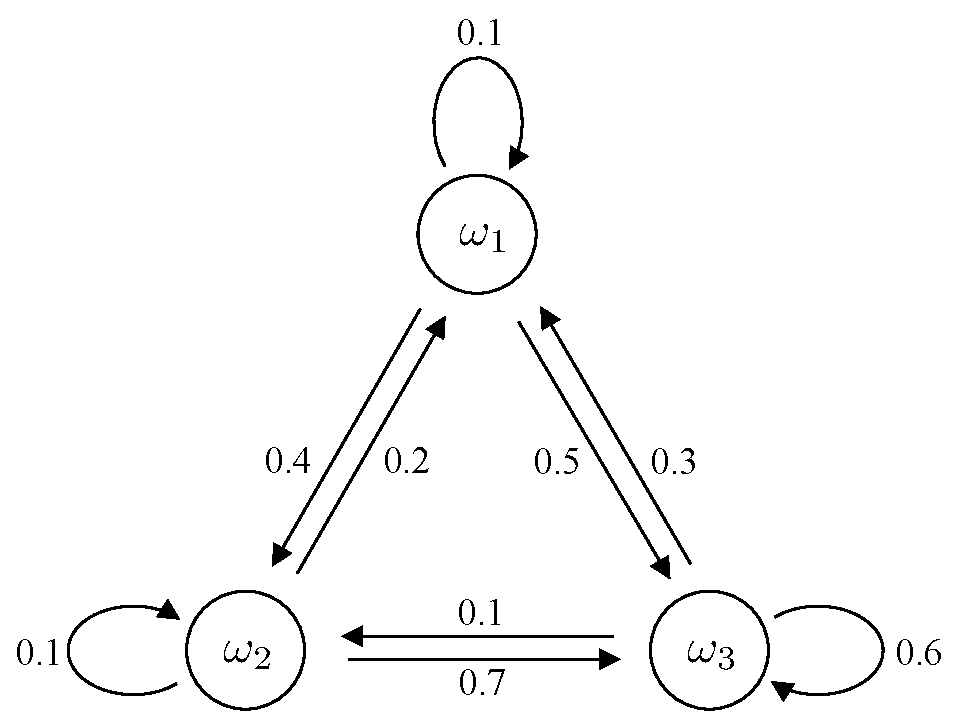
\includegraphics[width=\hsize, bb=0 0 461 344]{./fig/hidden_markov_model/markov_model.pdf}
		\subcaption{状態遷移図}
		\label{fig:markov:markovmodel1}
	\end{minipage}
	\begin{minipage}[t]{.5\hsize}
		\centering
		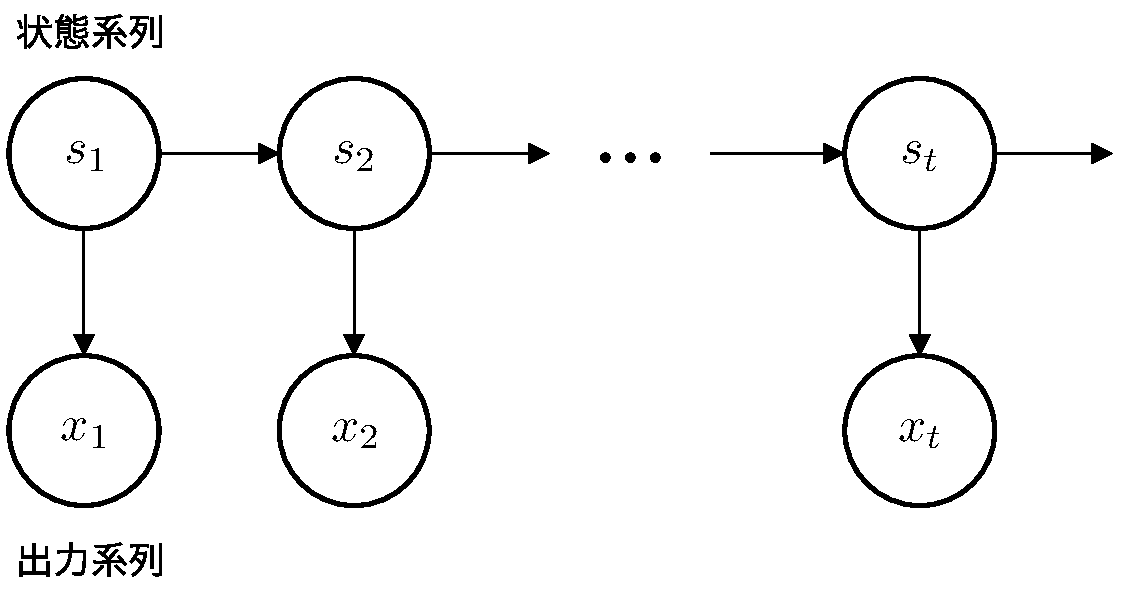
\includegraphics[width=\hsize, bb=0 0 551 289]{./fig/hidden_markov_model/markov_graph.pdf}
		\subcaption{状態空間モデル}
		\label{fig:markov:markovmodel2}
	\end{minipage}
	\caption{マルコフモデル}
	\label{fig:markov:markovmodel}
\end{figure}

\newpage

\section{隠れマルコフモデル}
\begin{sqbrrotnbr}{例題}
	\quad 箱の中に$c$種類のサイコロ$\omega_{1}, \omega_{2}, ..., \omega_{c},$があり,そのいずれかを取り出して投げ,出た目を観測した後,サイコロを元の箱に戻すという操作を$n$回繰り返す.
	ここで,
	\begin{enumerate}
		\item 最初にサイコロ$\omega_{i}$を取り出す確率は$\pi_{i}$である.
		\item サイコロ$\omega_{i}$を取り出した後にサイコロ$\omega_{j}$を取り出す確率は$a_{ij}$である.
		\item サイコロ$\omega_{j}$を投げて出た目が$v_{k}$となる確率は$b_{jk}$である.
	\end{enumerate}
	とする.
	ただし,$i,j=1,2,...,c,\ k=1,2,...,m$である.
	その結果,サイコロの目の系列として$\mathbf{x} = x_{1}x_{2} \cdots x_{t} \cdots x_{n}$が得られた.
	ただし,取り出したサイコロの種類については知ることができないものとする.

	\begin{enumerate}[label=(\arabic*)]
		\item パラメータ$\bm{A},\bm{B},\bm{\pi}$が既知のとき,このような観測結果が得られる確率$P(\mathbf{x})$を求めよ.
		% \item パラメータ$\bm{A},\bm{B},\bm{\pi}$が既知のとき,観測結果よりサイコロの種類の系列$\mathbf{s} = s_{1}s_{2} \cdots s_{t} \cdots s_{n}$を推定せよ.
		\item パラメータ$\bm{A},\bm{B},\bm{\pi}$が未知のとき,観測結果より,これらのパラメータを最尤推定により推定せよ.
	\end{enumerate}
\end{sqbrrotnbr}


\begin{myframe}{パラメータ}
	\begin{tabular}{ll}
		$c$ & :状態数 \\
		$m$ & :出力記号の数 \\
		$s_{t} \in \{\omega_{1}, \omega_{2},..., \omega_{c}\}$ & :時点$t$での状態 \\
		$x_{t} \in \{v_{1}, v_{2},..., v_{m}\}$ & :時点$t$での観測結果(出力記号) \\
		$\mathbf{s} = s_{1}s_{2}\cdots s_{t} \cdots s_{n}$ & :状態系列 \\
		$\mathbf{x} = x_{1}x_{2}\cdots x_{t} \cdots x_{n}$ & :観測記号系列 \\
		$a_{ij},a(\omega_{i}, \omega_{j})$ & :状態$\omega_{i}$から状態$\omega_{j}$への遷移確率 $P(\omega_{j} | \omega_{i})$ \\
		$b_{jk},b(\omega_{j}, v_{k})$ & :状態$\omega_{j}$で$v_{k}$を出力する確率 $P(v_{k} | \omega_{j})$\\
		$\pi_{i}$ & :初期状態($t=1$)が$\omega_{i}$である確率 $P(s_{1} = \omega_{i})$ \\
		$\bm{A}$ & :$a_{ij}$を($i,j$)成分としてもつ$c \times c$の行列 \\
		$\bm{B}$ & :$b_{jk}$を($j,k$)成分としてもつ$c \times m$の行列 \\
		$\bm{\pi}=(\pi_{1}, \pi_{2}, ..., \pi_{c})$ & :$\pi_{i}$を成分としてもつ$c$次元のベクトル
	\end{tabular}
\end{myframe}

この例題では,観測者はサイコロの投げた結果(出力記号)は知ることができるものの,サイコロの種類(状態)の系列を知ることができない.このようなモデルを\textbf{隠れマルコフモデル(Hidden Markov Model)}という.

例題(1)は,パラメータを既知としたとき,出力記号系列としての観測結果$\mathbf{x}$が得られる確率を求める\textbf{評価}の問題である.
% 例題(2)は,パラメータを既知としたとき,観測結果$\mathbf{x}$を導く可能性の最も高い状態系列を求める\textbf{復号}の問題である.
例題(2)は,パラメータを未知としたとき,観測結果から未知パラメータを求める\textbf{推定}の問題である.


\section{Forwardアルゴリズム}
例題(1)は,サイコロを投げた観測結果$\mathbf{x}$の生起確率$P(\mathbf{x})$を求める問題である.
観測できるのは$\mathbf{x}$のみであり,サイコロの種類の系列$\mathbf{s}$については知ることができないので,観測結果$\mathbf{x}$が得られたとき,$\mathbf{s}$としては可能な全ての系列を想定しなくてはならない.
すなわち,このような観測結果が得られる確率$P(\mathbf{x})$は,
\begin{equation}
P(\mathbf{x}) = \sum_{\mathbf{s}} P(\mathbf{x}, \mathbf{s}) \label{eq:px1}
\end{equation}
である.ここで$\displaystyle \sum_{\mathbf{s}}$は,
\begin{equation}
  \sum_{s_{1}}\sum_{s_{2}} \cdots \sum_{s_{n}}
\end{equation}
を表しており,可能な全ての系列$\mathbf{s}$についての和をとるという網羅的な演算である.
式(\ref{eq:px1})の$P(\mathbf{x}, \mathbf{s})$は確率の乗法定理より,
\begin{equation}
P(\mathbf{x}, \mathbf{s}) = P(\mathbf{x} | \mathbf{s}) P(\mathbf{s}) \label{eq:p_x_s_jyouhou}
\end{equation}
で表される.ここで,$P(\mathbf{x} | \mathbf{s}) $は,$\mathbf{s}$が与えられている前提があるため,
\begin{align}
P(\mathbf{x} | \mathbf{s}) & = P(x_{1} x_{2} \cdots x_{n} | s_{1} s_{2} \cdots s_{n}) \\
& = P(x_{1} | s_{1}) P(x_{2} | s_{2}) \cdots P(x_{n} | s_{n})
\end{align}
が成り立つので,
\begin{equation}
b(s_{t}, x_{t}) = P(x_{t} | s_{t})
\end{equation}
であることを用いて,
\begin{align}
P(\mathbf{x} | \mathbf{s}) & = b(s_{1}, x_{1}) b(s_{2}, x_{2}) \cdots b(s_{n}, x_{n}) \\
& = \prod_{t=1}^{n} b(s_{t}, x_{t}) \label{eq:p_x_g_s}
\end{align}
と書ける.一方,$ P(\mathbf{s})$は上記のような独立性は成り立たないが,
\begin{align}
P(\mathbf{s}) & = P(s_{1} s_{2} \cdots s_{n}) \\
& = P(s_{1}) a(s_{1}, s_{2}) a(s_{2}, s_{3}) \cdots a(s_{n-1}, s_{n}) \\
& = \prod_{t=1}^{n} a(s_{t-1}, s_{t}) \label{eq:p_s}
\end{align}
が成り立つ.ただし,
\begin{equation}
a(s_{0}, s_{1}) \overset{\mathrm{def}}{=} P(s_{1})
\end{equation}
である.式(\ref{eq:p_x_g_s})と式(\ref{eq:p_s})を式(\ref{eq:p_x_s_jyouhou})に代入することによって,
\begin{equation}
P(\mathbf{x}, \mathbf{s}) = \prod_{t=1}^{n} a(s_{t-1}, s_{t}) b(s_{t}, x_{t}) \label{eq:p_x_s}
\end{equation}
が得られる.よって式(\ref{eq:p_x_s})より,式(\ref{eq:px1})は,
\begin{equation}
  P(\mathbf{x}) = \sum_{\mathbf{s}} \prod_{t=1}^{n} a(s_{t-1}, s_{t}) b(s_{t}, x_{t}) \label{eq:px2}
\end{equation}
と表せる.ここで,式(\ref{eq:px2})の計算量について求めると,$O(nc^{n})$となる.これは膨大な計算が必要になり,この方法は非現実的である.

そこで,$P(\mathbf{x})$の効率的な計算方法について述べる.
まず,隠れマルコフモデルには以下の様な条件付き独立性が成立する\cite{PRLM_ge}.

\begin{mdframed}[topline = false, bottomline = false, rightline = false, innerlinewidth = 2pt, frametitle = 隠れマルコフモデルの条件付き独立性]
	\begin{enumerate}[label=(\arabic*)]
		\item $P(\mathbf{x} | s_{t}) = P(x_{1} \cdots x_{t} | s_{t}) P(x_{t+1} \cdots x_{n} | s_{t})$
    \item $P(x_{1} \cdots x_{t-1} | x_{t}, s_{t}) = P(x_{1} \cdots x_{t-1} | s_{t})$
    \item $P(x_{1} \cdots x_{t-1} | s_{t-1}, s_{t}) = P(x_{1} \cdots x_{t-1} | s_{t-1})$
    \item $P(x_{t+1} \cdots x_{n} | s_{t}, s_{t+1}) = P(x_{t+1} \cdots x_{n} | s_{t+1})$
    \item $P(x_{t+2} \cdots x_{n} | s_{t+1}, x_{t+1}) = P(x_{t+2} \cdots x_{n} | s_{t+1})$
    \item $P(\mathbf{x} | s_{t-1}, s{t}) = P(x_{1} \cdots x_{t-1} | s_{t-1}) P(x_{t} | s_{t}) P(x_{t+1} \cdots x_{n} | s_{t})$
    \item $P(x_{n+1} | \mathbf{x}, s_{n+1}) = P(x_{n+1} | s_{n+1})$
    \item $P(s_{n+1} | s_{n}, \mathbf{x}) = P(s_{n+1} | s_{n}) $
	\end{enumerate}
\end{mdframed}

観測結果$\mathbf{x} = x_{1}x_{2} \cdots x_{n}$が得られ,かつ$t$回目にサイコロ$\omega_{i}$を取り出している確率$P(\mathbf{x}, s_{t}=\omega_{i})$は,
確率の乗法定理と隠れマルコフモデルの条件付き独立性(1)より,
\begin{align}
P(\mathbf{x}, s_{t} = \omega_{i}) &= P(s_{t} = \omega_{i}) P(\mathbf{x} | s_{t} = \omega_{i}) \nonumber \\
& =  P(s_{t} = \omega_{i}) P(x_{1}x_{2} \cdots x_{t} | s_{t}=\omega_{i}) P(x_{t+1}x_{t+2} \cdots x_{n}|s_{t}=\omega_{i}) \nonumber \\
& =  P(x_{1}x_{2} \cdots x_{t}, s_{t}=\omega_{i}) P(x_{t+1}x_{t+2} \cdots x_{n}|s_{t}=\omega_{i}) \nonumber \\
& = \alpha_{t}(i) \beta_{t}(i) \label{eq:pxsaiteki}
\end{align}
と書ける.
ここで,$\alpha_{t}(i)$,$\beta_{t}(i)$は
\begin{align}
\alpha_{t}(i) & \overset{\mathrm{def}}{=}  P(x_{1}x_{2} \cdots x_{t}, s_{t}=\omega_{i}) \label{eq:alpha}\\
\beta_{t}(i)  & \overset{\mathrm{def}}{=}  P(x_{t+1}x_{t+2} \cdots x_{n}|s_{t}=\omega_{i})  \label{eq:beta}
\end{align}
とした.
$\alpha_{t}(i)$は,$x_{1}x_{2}\cdots x_{t}$という観測結果が得られ,かつ$t$回目にサイコロ$\omega_{i}$を取り出している確率である.
一方,$\beta_{t}(i)$は,$t$回目にサイコロ$\omega_{i}$を取り出したという条件のもとで,それ以降の観測結果が$x_{t+1}x_{t+2} \cdots x_{n}$となる確率である.
すなわち,式(\ref{eq:pxsaiteki})では,$t$回目までの観測結果までと,それより後の観測結果とに分けて考えている.

ここで,$\alpha_{t}(i)$は,次式で示すように再帰的な計算方法で求めることができる.
\begin{align}
  \alpha_{t}(j) & = P(x_{1} x_{2} \cdots x_{t-1} x_{t}, s_{t}=\omega_{j}) \\
  % \intertext{$x_{1} x_{2} \cdots x_{t-1}$を$\mathbf{x}^{t-1}_{1}$とすると,}
  & = P(x_{1} x_{2} \cdots x_{t} | s_{t} = \omega_{j}) P(s_{t} = \omega_{j}) \\
  & = P(x_{t} | s_{t} = \omega_{j}) P(x_{1} x_{2} \cdots x_{t-1} | s_{t} = \omega_{j}) P(s_{t} = \omega_{j}) \\
  & = P(x_{t} | s_{t} = \omega_{j}) P(x_{1} x_{2} \cdots x_{t-1}, s_{t} = \omega_{j}) \\
  \intertext{$P(x_{t} | s_{t} = \omega_{j}) = b(\omega_{j}, x_{t})$より,}
  & = b(\omega_{j}, x_{t}) \sum_{s_{t-1}} P(x_{1} x_{2} \cdots x_{t-1}, s_{t-1}, s_{t} = \omega_{j}) \\
  & = b(\omega_{j}, x_{t}) \sum_{s_{t-1}} P(x_{1} x_{2} \cdots x_{t-1}, s_{t} = \omega_{j} | s_{t-1}) P(s_{t-1}) \\
  & = b(\omega_{j}, x_{t}) \sum_{s_{t-1}} P(x_{1} x_{2} \cdots x_{t-1} | s_{t-1}) P(s_{t} = \omega_{j} | s_{t-1}) P(s_{t-1}) \\
  & = b(\omega_{j}, x_{t}) \sum_{s_{t-1}} P(x_{1} x_{2} \cdots x_{t-1} , s_{t-1}) P(s_{t} = \omega_{j} | s_{t-1}) \\
  & = b(\omega_{j}, x_{t}) \sum_{i=1}^{c} P(x_{1} x_{2} \cdots x_{t-1} , s_{t-1} = \omega_{i}) P(s_{t} = \omega_{j} | s_{t-1} = \omega_{i}) \\
  \intertext{式(\ref{eq:alpha})と$P(s_{t} = \omega_{j} | s_{t-1} = \omega_{i}) = a_{ij}$より,}
  & = b(\omega_{j}, x_{t}) \sum_{i=1}^{c} \alpha_{t-1}(i) a_{ij}
\end{align}

よって,
\begin{align}
\alpha_{t}(j) = b(\omega_{j}, x_{t}) \sum_{i=1}^{c} \alpha_{t-1}(i) a_{ij} \label{eq:forward_saiki_shiki} \\
(t=2,3,...,n) \quad (j=1,2,...,c) \nonumber
\end{align}
ただし,
\begin{align}
\alpha_{1}(i) &= P(x_{1}, s_{1} = \omega_{i}) \nonumber \\
&= P(s_{1} = \omega_{i})P(x_{1} | s_{1} = \omega_{i}) \nonumber \\
&= \pi_{i} b(\omega_{i}, x_{1}) \quad (i = 1,2,...,c)
\end{align}
である.

観測順と同じ方向に向かって順次$\alpha_{t}(j)$を求めていることから,このような計算方法\textbf{前向きアルゴリズム(Forward algorithm)}と呼ぶ\cite{zokupata}.
%Forwardアルゴリズムの計算式(\ref{eq:forward_saiki_shiki})の構造が図\ref{fig:markov:forward}に示されている.

ここで,式(\ref{eq:alpha})において,$t=n$とすることにより,
\begin{equation}
\alpha_{n}(i) = P(x_{1}x_{2} \cdots x_{n}, s_{n} = \omega_{i}) \label{eq:alpha_teigi}
\end{equation}
が得られ,式(\ref{eq:alpha_teigi})の同時確率を$s_{n}$について周辺化することにより,求める$P(\mathbf{x})$は
\begin{equation}
P(\mathbf{x}) = \sum_{i=1}^{c} \alpha_{n}(i) \label{eq:forward_px}
\end{equation}
となる.
この計算量は$O(c^{2}n)$であり,先ほどと比較すればその効率性は明らかである.

Forwardアルゴリズムの手順をAlgorithm \ref{alg:forward}に示す.
%\begin{figure}[htb]
%	\centering
%	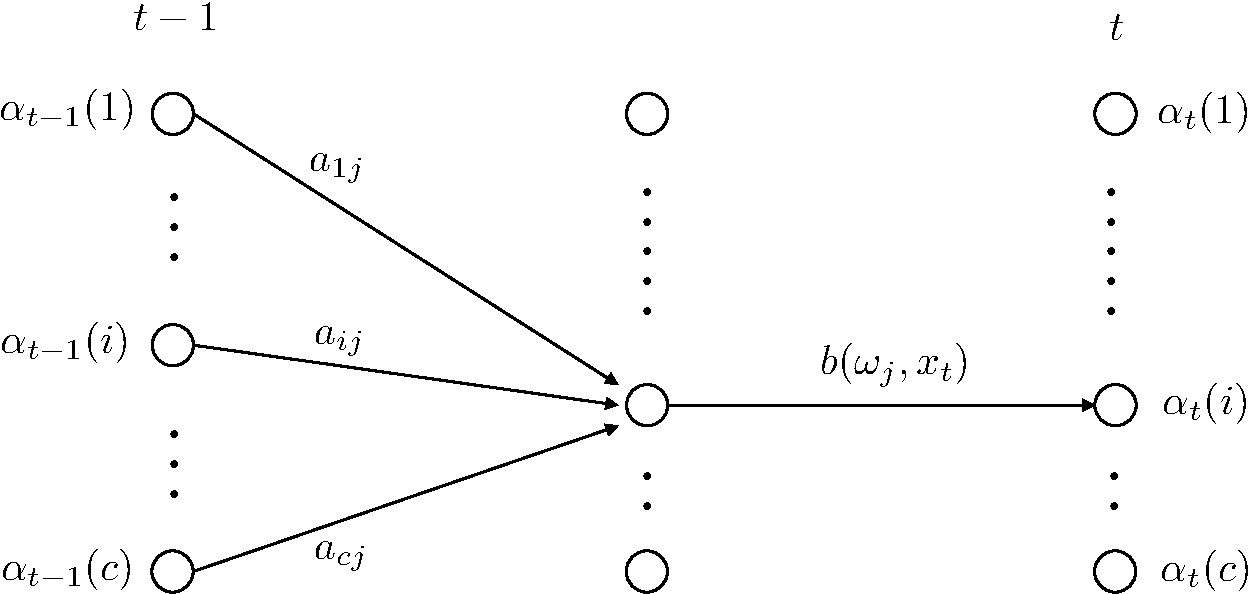
\includegraphics[width=.9\hsize]{forward.pdf}
%	\caption{前向きアルゴリズム}
%	\label{fig:markov:forward}
%\end{figure}

\begin{algorithm}[H]
		\caption{Forward algorithm}
		\label{alg:forward}
		\begin{algorithmic}
			\STATE \textbf{Step 1 初期化}
			\STATE \quad $\alpha_{1}(i)  = \pi_{i} b(\omega_{i}, x_{1}) \quad (i = 1,2,...,c)$
			\STATE \textbf{Step 2 再帰的計算}
			\STATE \quad $\displaystyle \alpha_{t}(j) = b(\omega_{j}, x_{t}) \sum_{i=1}^{c} \alpha_{t-1}(i) a_{ij} \qquad(t=2,3,...,n) \quad (j=1,2,...,c)$
			\STATE \textbf{Step 3 確率の計算}
			\STATE \quad $\displaystyle P(\mathbf{x}) = \sum_{i=1}^{c} \alpha_{n}(i)$
		\end{algorithmic}
\end{algorithm}


\section{Backwardアルゴリズム}
Forwardアルゴリズムは$\alpha_{t}(i)$から$P(\mathbf{x})$を求めたが,$\beta_{t}(i)$を用いても同様に$P(\mathbf{x})$を求めることができる.
これを\textbf{後向きアルゴリズム(Backward algorithm)}と呼ぶ.

$\alpha_{t}(i)$と同様に,$\beta_{t}(i)$も次式で示すように再帰的な計算方法で求めることができる.
\begin{align}
	\beta_{t}(i) &= P(x_{t+1} x_{t+2} \cdots x_{n} | s_{t} = \omega_{i}) \\
	&= \sum_{s_{t+1}} P(x_{t+1} x_{t+2} \cdots x_{n}, s_{t+1} | s_{t} = \omega_{i}) \\
	&= \sum_{s_{t+1}} P(x_{t+1} x_{t+2} \cdots x_{n} | s_{t+1}, s_{t} = \omega_{i}) P(s_{t+1} | s_{t} = \omega_{i}) \\
	\intertext{隠れマルコフモデルの条件付き独立性(4)より,}
	&= \sum_{s_{t+1}} P(x_{t+1} x_{t+2} \cdots x_{n} | s_{t+1}) P(s_{t+1} | s_{t} = \omega_{i}) \\
	&= \sum_{s_{t+1}} P(x_{t+2} x_{t+3} \cdots x_{n} | s_{t+1}) P(x_{t+1} | s_{t+1}) P(s_{t+1} | s_{t} = \omega_{i}) \\
	&= \sum_{j=1}^{c} P(x_{t+2} x_{t+3} \cdots x_{n} | s_{t+1} = \omega_{j}) P(x_{t+1} | s_{t+1} = \omega_{j}) P(s_{t+1} = \omega_{j} | s_{t} = \omega_{i}) \\
	\intertext{式(\ref{eq:beta})と$P(s_{t} = \omega_{j} | s_{t-1} = \omega_{i}) = a_{ij}$,$P(x_{t} | s_{t} = \omega_{j}) = b(\omega_{j}, x_{t})$より,}
	&= \sum_{j=1}^{c} a_{ij} b(\omega_{j}, x_{t+1}) \beta_{t+1}(j)
\end{align}
よって,
\begin{align}
	\beta_{t}(i) =  \sum_{j=1}^{c} a_{ij} b(\omega_{j}, x_{t+1}) \beta_{t+1}(j) \\
	(t=2,3,...,n) \quad (j=1,2,...,c) \nonumber
\end{align}
ただし,
\begin{equation}
\beta_{n}(i) = 1 \quad (i = 1,2,...,c)
\end{equation}
である.

$\beta_{t}(i)$を用いて$P(\mathbf{x})$を求める方法を考えてみる.
まず,式(\ref{eq:beta})において,$t=1$とすることにより,
\begin{equation}
\beta_{1}(i) = P(x_{2} x_{3} \cdots x_{n} | s_{1} = \omega_{i})
\end{equation}
が得られる.
\begin{align}
	P(x_{1} x_{2} \cdots x_{n} | s_{1} = \omega_{i}) & = P(x_{1} | s_{1} = \omega_{i}) P(x_{2} x_{3} \cdots x_{n} | s_{1} = \omega_{i}) \\
	& = b(\omega_{i}, x_{1}) \beta_{1}(i)
\end{align}
であるから,求めたい$P(\mathbf{x})$は
\begin{align}
  P(\mathbf{x}) & = \sum^{c}_{i=1} P(x_{1} x_{2} \cdots x_{n}, s_{1} = \omega_{i}) \\
  & = \sum^{c}_{i=1} P(s_{1} = \omega_{i} )P(x_{1} x_{2} \cdots x_{n} | s_{1} = \omega_{i}) \\
  & = \sum_{i=1}^{c} \pi_{i} b(\omega_{i}, x_{1}) \beta_{1}(i)
\end{align}
となる.

Backwardアルゴリズムの手順をAlgorithm \ref{alg:backward}に示す.

\begin{algorithm}
		\caption{Backward algorithm}
		\label{alg:backward}
		\begin{algorithmic}
			\STATE \textbf{Step 1 初期化}
			\STATE \quad $\beta_{n}(i) = 1 \quad (i = 1,2,...,c)$
			\STATE \textbf{Step 2 再帰的計算}
			\STATE \quad $\displaystyle \beta_{t}(i) = \sum_{j=1}^{c} a_{ij} b(\omega_{j}, x_{t+1}) \beta_{t+1}(j) \qquad (t=(n-1),...,2,1) \quad (i=1,2,...,c)$
			\STATE \textbf{Step 3 確率の計算}
			\STATE \quad $\displaystyle P(\mathbf{x}) = \sum_{i=1}^{c} \pi_{i} b(\omega_{i}, x_{1}) \beta_{1}(i)$
		\end{algorithmic}
\end{algorithm}


\newpage


\section{Baum-Welchアルゴリズム}
ここではまず準備として,次のような$\gamma_{t}(i), \xi_{t}(i, j)$を定義する.
\begin{align}
	\gamma_{t}(i) \overset{\mathrm{def}}{=} P(s_{t} & = \omega_{i} | \mathbf{x}) \label{eq:def_gamma} \\
	\xi_{t}(i, j) \overset{\mathrm{def}}{=} P(s_{t} & = \omega_{i}, s_{t+1} = \omega_{j}| \mathbf{x}) \label{eq:xi}
\end{align}

上式の$\gamma_{t}(i)$は,観測結果\textbf{x}が得られたという条件で,$t$回目にサイコロ$\omega_{i}$を取り出している確率である.よって,
\begin{equation}
\sum_{i=1}^{c} \gamma_{t}(i) = 1
\end{equation}
が成り立つ.

式(\ref{eq:def_gamma})に式(\ref{eq:pxsaiteki}),(\ref{eq:forward_px})を適用することにより,$\gamma_{t}(i)$は
\begin{align}
	\gamma_{t}(i) & = P(s_{t} = \omega_{i} | \mathbf{x}) \nonumber \\
	& = \frac{P(\mathbf{x}, s_{t}=\omega_{i})}{P(\mathbf{x})} \nonumber \\
	& = \frac{\alpha_{t}(i) \beta_{t}(i)}{\displaystyle \sum_{i=1}^{c} \alpha_{n}(i)}
\end{align}
と表される.

式(\ref{eq:xi})は,観測結果$\mathbf{x} = x_{1}x_{2}\cdots x_{n}$が得られたという条件で,$t$回目にサイコロ$\omega_{i}$を,$(t+1)$回目にサイコロ$\omega_{j}$を取り出している確率を表している.

また,以下の式が成り立つ.
\begin{align}
\sum_{j=1}^{c} \xi_{t}(i, j) & = \sum_{j=1}^{c} P(s_{t} = \omega_{i}, s_{t+1} = \omega_{j}| \mathbf{x}) \\
& = P(s_{t} = \omega_{i} | \mathbf{x}) \\
& = \gamma_{t}(i) \label{eq:xi_gamma}
\end{align}

ここで,$\mathbf{x} = x_{1}x_{2}\cdots x_{n}$が観測され,かつ$t$回目にサイコロ$\omega_{i}$を,$(t+1)$回目にサイコロ$\omega_{j}$を取り出している確率$P(\mathbf{x}, s_{t} = \omega_{i}, s_{t+1} = \omega_{j})$を求めると,
\begin{align}
	P(\mathbf{x}&, s_{t} = \omega_{i}, s_{t+1} = \omega_{j}) \nonumber \\
	& = P(\mathbf{x} | s_{t} = \omega_{i}, s_{t+1} = \omega_{j}) \cdot P(s_{t} = \omega_{i}, s_{t+1} = \omega_{j}) \nonumber \\
	\intertext{隠れマルコフモデルの条件付き独立性(6)より,}
	& = P(x_{1}x_{2}\cdots x_{t} | s_{t} = \omega_{i}) \cdot P(x_{t+1} | s_{t+1} = \omega_{j} ) \cdot P(x_{t+2} \cdots x_{n} | s_{t+1} = \omega_{j}) \cdot P(s_{t+1} = \omega_{j} | s_{t} = \omega_{i}) \cdot P(s_{t} = \omega_{i})  \nonumber \\
	& = P(x_{1}x_{2}\cdots x_{t}, s_{t} = \omega_{i}) \cdot P(s_{t+1} = \omega_{j} | s_{t} = \omega_{i} ) \cdot P(x_{t+1} | s_{t+1} = \omega_{j} ) \cdot P(x_{t+2} \cdots x_{n} | s_{t+1} = \omega_{j}) \nonumber \\
	& = \alpha_{t}(i) a_{ij} b(\omega_{j}, x_{t+1}) \beta_{t+1}(j)
\end{align}
となる.これより
\begin{align}
\xi_{t}(i, j) & = P(s_{t} = \omega_{i}, s_{t+1} = \omega_{j}| \mathbf{x}) \\
& = \frac{P(\mathbf{x}, s_{t} = \omega_{i}, s_{t+1} = \omega_{j})}{P(\mathbf{x})} \\
& = \frac{\alpha_{t}(i) a_{ij} b(\omega_{j}, x_{t+1}) \beta_{t+1}(j)}{\displaystyle \sum_{i=1}^{c} \alpha_{n}(i)}
\end{align}
が得られる.

これらの結果をもとに,最尤推定を用いてパラメータ推定を行う.推定すべきパラメータ$\bm{A},\bm{B},\bm{\pi}$をまとめて
\begin{equation}
\bm{\theta} = (\bm{A},\bm{B},\bm{\pi})
\end{equation}
とする.

最尤推定により最適なパラメータ$\bm{\theta}$を求めることは,$P(\mathbf{x}; \bm{\theta})$を$\bm{\theta}$に関して最大化することである.
そのためにはEMアルゴリズムを適用し,Q関数を最大化すれば良い.

\begin{equation}
Q(\bm{\theta}^{0}, \bm{\theta}) = \sum_{\mathbf{s}} P(\mathbf{s} | \mathbf{x}; \bm{\theta}^{0}) \log P(\mathbf{x}, \mathbf{s}; \bm{\theta}) \label{eq:Qfunc}
\end{equation}

ここで,$\bm{\theta}$は$\bm{\theta}^{0}$を更新した結果得られる新しいパラメータである.Q関数を最大化するには,パラメータを繰り返し更新すればよい.

式(\ref{eq:Qfunc})の右辺の$P(\mathbf{x}, \mathbf{s}; \bm{\theta})$は確率の乗法定理より,
\begin{align}
P(\mathbf{x}, \mathbf{s}; \bm{\theta}) & = P(\mathbf{s}; \bm{\theta}) P(\mathbf{x} | \mathbf{s}; \bm{\theta})
\intertext{と表せる.両辺の対数をとると,}
\log P(\mathbf{x}, \mathbf{s}; \bm{\theta}) & = \log P(\mathbf{s}; \bm{\theta}) + \log P(\mathbf{x} | \mathbf{s}; \bm{\theta}) \\
\intertext{ここで,式(\ref{eq:p_x_g_s})と式(\ref{eq:p_s})を用いると}
& = \log P(s_{1}) + \sum_{t=1}^{n-1} \log a(s_{t}, s_{t+1}) + \sum_{t=1}^{n}\log b(s_{t}, x_{t})
\end{align}
が得られる.
したがって,式(\ref{eq:Qfunc})より,
\begin{align}
Q(\bm{\theta}^{0}, \bm{\theta}) & = \sum_{\mathbf{s}} P(\mathbf{s} | \mathbf{x}; \bm{\theta}^{0}) \log P(s_{1}) + \sum_{\mathbf{s}} P(\mathbf{s} | \mathbf{x}; \bm{\theta}^{0}) \sum_{t=1}^{n-1} \log a(s_{t}, s_{t+1}) + \sum_{\mathbf{s}} P(\mathbf{s} | \mathbf{x}; \bm{\theta}^{0}) \sum_{t=1}^{n}\log b(s_{t}, x_{t}) \\
& = Q(\bm{\theta}^{0}, \bm{\pi}) + Q(\bm{\theta}^{0}, \bm{A}) + Q(\bm{\theta}^{0}, \bm{B})
\end{align}
となる.ここで,
\begin{align}
Q(\bm{\theta}^{0}, \bm{\pi}) & \overset{\mathrm{def}}{=} \sum_{\mathbf{s}} P(\mathbf{s} | \mathbf{x}; \bm{\theta}^{0}) \log P(s_{1}) \\
Q(\bm{\theta}^{0}, \bm{A}) & \overset{\mathrm{def}}{=} \sum_{\mathbf{s}} P(\mathbf{s} | \mathbf{x}; \bm{\theta}^{0}) \sum_{t=1}^{n-1} \log a(s_{t}, s_{t+1}) \\
Q(\bm{\theta}^{0}, \bm{B}) & \overset{\mathrm{def}}{=} \sum_{\mathbf{s}} P(\mathbf{s} | \mathbf{x}; \bm{\theta}^{0}) \sum_{t=1}^{n}\log b(s_{t}, x_{t}) \label{eq:Q_B}
\end{align}
と定義した.上の3式は,それぞれパラメータ$\bm{\pi},\bm{A},\bm{B}$のみを含む.したがって,$Q(\bm{\theta}^{0}, \bm{\theta})$を$\bm{\theta}$について最大化するには,$Q(\bm{\theta}^{0}, \bm{\pi}),Q(\bm{\theta}^{0}, \bm{A}),Q(\bm{\theta}^{0}, \bm{B})$を,それぞれパラメータ$\bm{\pi},\bm{A},\bm{B}$について最大化すればよい.ここで,$\bm{\theta}^{0}$は更新前のパラメータであるので,最大化に当たっては定数とみなしてよい.

\subsection*{$\bm{Q(\theta}^{0}, \bm{A)}$の最大化}
$Q(\bm{\theta}^{0}, \bm{A})$は,
\begin{equation}
Q(\bm{\theta}^{0}, \bm{A}) = \sum_{s_{1}} \cdots \sum_{s_{n}} P(s_{1} \cdots s_{n} | \mathbf{x}; \bm{\theta}^{0}) \sum_{t=1}^{n-1} \log a(s_{t}, s_{t+1})
\end{equation}
と書ける.上式の加算部分に現れるペア$(s_{t}, s_{t+1})$の中には,$t$が異なっていても同じ内容$(\omega_{i}, \omega_{j})$を持つものが含まれている.そこで.上式を$\log a_{ij}(=\log a(\omega_{i}, \omega_{j}))$でくくりだして整理すると,
\begin{equation}
Q(\bm{\theta}^{0}, \bm{A}) = \sum_{i=1}^{c} \sum_{j=1}^{c} \left( \sum_{t=1}^{n-1} \sum_{\substack{\mathbf{s} \\ (s_{t} = \omega_{i}) \\ (s_{t+1} = \omega_{j})}} P(s_{1} \cdots s_{n} | \mathbf{x}; \bm{\theta}^{0}) \right) \log a_{ij} \label{eq:max_A_1}
\end{equation}
となる.ただし,上式で$\mathbf{s}$についての加算は,
\begin{equation}
\mathbf{s} = s_{1} s_{2} \cdots \overset{(t)}{\omega_{i}} \overset{(t+1)}{\omega_{j}} \cdots s_{n}
\end{equation}
のように,$s_{t}=\omega_{i}$,$s_{t+1} = \omega_{j}$を満たす全ての$\mathbf{s}$について実行することを示している.
ここで,式(\ref{eq:xi})を用いると,式(\ref{eq:max_A_1})において,
\begin{align}
\sum_{\substack{\mathbf{s} \\ (s_{t} = \omega_{i}) \\ (s_{t+1} = \omega_{j})}} P(s_{1} \cdots s_{n} | \mathbf{x}; \bm{\theta}^{0}) & = P(s_{t} = \omega_{i}, s_{t+1} = \omega_{j} | \mathbf{x}; \bm{\theta}) \\
& = \xi_{t}(i, j)
\end{align}
が成り立つ.この結果より,
\begin{align}
Q(\bm{\theta}^{0}, \bm{A}) & = \sum_{i=1}^{c} \sum_{j=1}^{c} \left( \sum_{t=1}^{n-1} \xi_{t} (i, j) \right) \log a_{ij} \\
& = \sum_{i=1}^{c} \left( \sum_{j=1}^{c} c_{ij} \log a_{ij} \right) \label{eq:max_A_2}
\end{align}
となる.ここで,
\begin{equation}
c_{ij} \overset{\mathrm{def}}{=} \sum_{t=1}^{n-1} \xi_{t} (i, j)
\end{equation}
と定義した.
上記$c_{ij}$は,更新前のパラメータ$\bm{\theta}^{0}$に基づいて計算されるので,$\bm{A}$に関する最大化に際しては定数として扱える.

式(\ref{eq:max_A_2})を最大化するには,各$i$ごとに,
\begin{equation}
\sum_{j=1}^{c} c_{ij} \log a_{ij} \qquad (i = 1, 2, ..., c) \label{eq:max_A_3}
\end{equation}
を最大化すればよい.ここで,
\begin{equation}
\sum_{j=1}^{c} a_{ij} = 1 \qquad (i = 1, 2, ..., c) \label{eq:max_A_4}
\end{equation}
が成立するので,式(\ref{eq:max_A_4})の条件の下で式(\ref{eq:max_A_3})を最大にする$a_{ij}$を推定値$\hat{a}_{ij}$とすると,以下の定理が使える.

\begin{mdframed}[topline = false, bottomline = false, rightline = false, innerlinewidth = 2pt, frametitle = 定理1]
	いま,$n$個の正の定数$w_{1},w_{2},...,w_{n}$がある.\\
	ここで,$n$個の変数$x_{1}, x_{2}, ..., x_{n} \ (0 < x_{i} < 1)$が,拘束条件
	\begin{equation}
	\sum_{i = 1}^{n} x_{i} = 1
	\end{equation}
	を満たしているものとする.このとき,
	\begin{equation}
	f(x_{1}, x_{2}, ..., x_{n}) = \sum_{i = 1}^{n} w_{i} \log x_{i}
	\end{equation}
	を最大にする$x_{i}$は次式で与えられる.
	\begin{equation}
	x_{i} = \frac{w_{i}}{ \displaystyle \sum_{k=1}^{n} w_{k}} \qquad (i = 1, 2, ..., n)
	\end{equation}
\end{mdframed}

この定理を用いると,
\begin{equation}
\hat{a}_{ij} = \frac{c_{ij}}{\displaystyle \sum_{i=1}^{c} c_{ij}} \label{eq:A_hat}
\end{equation}
である.この式の分母は,式(\ref{eq:xi_gamma})を用いることにより,
\begin{equation}
\sum_{j=1}^{c} c_{ij} = \sum_{j=1}^{c} \sum_{t=1}^{n-1} \xi_{t} (i, j) = \sum_{t=1}^{n-1} \gamma_{t}(i)
\end{equation}
であるので,式(\ref{eq:A_hat})は下式のように書ける.
\begin{equation}
\hat{a}_{ij} = \frac{\displaystyle \sum_{t=1}^{n-1} \xi_{t} (i, j)}{\displaystyle \sum_{t=1}^{n-1} \gamma_{t} (i)}
\end{equation}

ここで,上式の妥当性について考察する.式(\ref{eq:def_gamma}),(\ref{eq:xi})で示した$\gamma_{t}(i)$および$\xi_{t}(i, j)$の定義より,上式の分母,分子は,観測結果$\mathbf{x}$が得られたという条件の下でそれぞれ以下の値を計算していることがわかる.
\begin{align*}
\sum_{t=1}^{n-1} \gamma_{t} (i) & = サイコロ\omega_{i}を取り出した回数の期待値 \\
& = 状態\omega_{i}となった回数の期待値 \\
\sum_{t=1}^{n-1} \xi_{t} (i, j) & = サイコロ\omega_{i}の次に\omega_{j}を取り出した回数の期待値 \\
& = 状態\omega_{i}から状態\omega_{j}へ遷移した回数の期待値
\end{align*}
したがって,$a_{ij}$の推定値として,式(\ref{eq:A_hat})を用いるのは妥当である.



\subsection*{$\bm{Q(\theta}^{0}, \bm{B)}$の最大化}
上で述べた方法と同様に,式(\ref{eq:Q_B})についても,$(s_{t}, x_{t})$のペアの中で,同じ内容$(\omega_{j}, v_{k})$であるものをまとめるため,$\log b_{jk}$でくくりだして整理すると,$Q(\bm{\theta}^{0}, \bm{B})$は
\begin{align}
Q(\bm{\theta}^{0}, \bm{B}) & = \sum_{\bm{s}} P(\bm{s} | \mathbf{x}; \bm{\theta}^{0}) \sum_{t=1}^{n} \log b(s_{t}, x_{t}) \\
& = \sum_{s_{1}} \cdots \sum_{s_{n}} P(s_{1} \cdots s_{n} | x_{1} \cdots x_{n}; \bm{\theta}^{0}) \sum_{t~1}^{n} \log b(s_{t}, x_{t}) \\
& =  \sum_{j=1}^{c} \sum_{k=1}^{m} \left( \sum_{t=1}^{n} \delta (x_{t}, v_{k})  \sum_{\substack{\mathbf{s} \\ (s_{t} = \omega_{i})}} P(s_{1} \cdots s_{n} | x_{1} \cdots x_{n}; \bm{\theta}^{0}) \right) \log b_{jk} \label{eq:QB_kukuri}
\end{align}
と表される.
ただし,上式で$\bm{s}$についての加算は,$s_{t} = \omega_{j}$を満たすすべての$\bm{s}$について実行することを示している.
また,$\delta(x_{t}, v_{k})$は,$P(s_{1}\cdots s_{n} | x_{1} \cdots x_{n})$の中から$x_{t} = v_{k}$を満たすもののみを抽出するための項であり,
\begin{equation}
\delta(x_{t}, v_{k}) = \left\{ \begin{array}{ll}
1 & (x_{t} = v_{k}) \\
0 & \mathit{(otherwise)}
\end{array} \right.
\end{equation}
である.
式(\ref{eq:def_gamma})を用いると,式(\ref{eq:QB_kukuri})において,
\begin{align}
 \sum_{\substack{\mathbf{s} \\ (s_{t} = \omega_{i})}} P(s_{1} \cdots s_{n} | x_{1} \cdots x_{n}; \bm{\theta}^{0}) & = P(s_{t} = \omega_{j} | \mathbf{x}; \bm{\theta}^{0}) \\
 & = \gamma_{t}(j)
\end{align}
が成り立つ.
この結果より,式(\ref{eq:QB_kukuri})は
\begin{align}
	Q(\bm{\theta}^{0}, \bm{B}) & = \sum^{c}_{j=1} \sum^{m}_{k=1} \left( \sum_{t=1}^{n} \delta (x_{t}, v_{k}) \gamma_{t}(j) \right) \log b_{jk} \\
	& = \sum^{c}_{j=1} \left( \sum^{m}_{k=1} d_{jk} \log b_{jk} \right) \label{eq:QB_henkei_last}
\end{align}
と表される.ここで,
\begin{equation}
d_{jk} \overset{\mathrm{def}}{=} \sum_{t=1}^{n} \delta (x_{t}, v_{k}) \gamma_{t}(j)
\end{equation}
と定義した.
これまで同様,$d_{jk}$はパラメータ$\bm{\theta}^{0}$にのみ依存するので,定数として扱える.
式(\ref{eq:QB_henkei_last})を最大化するためには,各$j$ごとに
\begin{equation}
\sum^{m}_{k=1} d_{jk} \log b_{jk} \label{eq:QB_target_func}
\end{equation}
を最大化すればよい.
出力確率$b_{jk}$は
\begin{equation}
\sum^{m}_{k=1} b_{jk} = 1 \qquad (j = 1,2,...,c) \label{eq:emission_sum_1}
\end{equation}
が成り立つので,式(\ref{eq:emission_sum_1})の条件のもとで式(\ref{eq:QB_target_func})を最大にする$b_{jk}$を推定値$\hat{b_{jk}}$とすると,定理1より
\begin{equation}
\hat{b}_{jk} = \frac{d_{jk}}{\displaystyle \sum_{l=1}^{m} d_{jl}} \label{eq:bjk_hat}
\end{equation}
と求めることができる.式(\ref{eq:bjk_hat})は
\begin{align}
 \sum_{l=1}^{m} d_{jl}  & = \sum_{l=1}^{m}\sum_{t=1}^{n} \delta(x_{t}, v_{l}) \gamma_{t}(j) \\
 & = \sum_{t=1}^{n} \gamma_{t}(j) \sum_{l=1}^{m} \delta(x_{t}, v_{l}) \\
 & =  \sum_{t=1}^{n} \gamma_{t}(j)
\end{align}
である.
よって推定値$\hat{b}_{jk}$は次のようになる.
\begin{equation}
\hat{b}_{jk} = \frac{\displaystyle \sum_{t=1}^{n} \delta (x_{t}, v_{k}) \gamma_{t}(j)}{\displaystyle \sum_{t=1}^{n} \gamma_{t}(j)}
\end{equation}


\subsection*{$\bm{Q(\theta}^{0}, \bm{\pi)}$の最大化}
これまでと同様に
\begin{align}
Q(\bm{\theta}^{0}, \bm{\pi}) & = \sum_{\mathbf{s}} P(\mathbf{s} | \mathbf{x}; \bm{\theta}^{0}) \log P(s_{1}) \\
& = \sum_{s_{1}} \cdots \sum_{s_{n}} P(s_{1} \cdots s_{n} | \mathbf{x}; \bm{\theta}^{0})  \log P(s_{1})  \\
& =  \sum_{i=1}^{c} \left( \sum_{\substack{\mathbf{s} \\ (s_{1} = \omega_{i})}} P(s_{1} \cdots s_{n} | \mathbf{x}; \bm{\theta}^{0}) \right) \log P(s_{1} = \omega_{i}) \label{eq:QPI_henkei1}
\end{align}
となる.
ここで,
\begin{equation}
\sum_{\substack{\mathbf{s} \\ (s_{1} = \omega_{i})}} P(s_{1} \cdots s_{n} | \mathbf{x}; \bm{\theta}^{0}) = P(s_{1} = \omega_{i} | \mathbf{x};  \bm{\theta}^{0})
\end{equation}
であり,
\begin{equation}
P(s_{1} = \omega_{i}) = \pi_{i}
\end{equation}
が成り立つので,これらを式(\ref{eq:QPI_henkei1})に代入することにより
\begin{align}
Q(\bm{\theta}^{0}, \bm{\pi}) & = \sum_{i=1}^{c} P(s_{1} = \omega_{i} | \mathbf{x}; \bm{\theta}^{0}) \cdot \log \pi_{i} \\
& = \sum_{i=1}^{c} e_{i} \log \pi_{i} \label{eq:Q_PI_last}
\end{align}
を得る.
ここで
\begin{equation}
e_{i} \overset{\mathrm{def}}{=} P(s_{1} = \omega_{i} | \mathbf{x}; \bm{\theta}^{0}) \label{eq:def_ei}
\end{equation}
と定義した.
これも更新前のパラメータ$\bm{\theta}^{0}$のみに依存し,定数として扱える.

初期確率$\pi_{i}$は,
\begin{equation}
\sum_{i=1}^{c} \pi_{i} = 1 \label{eq:init_prob_sum}
\end{equation}
である.
式(\ref{eq:init_prob_sum})のもとで式(\ref{eq:Q_PI_last})を最大にする$\pi_{i}$を推定値$\hat{\pi}_{i}$とすると,ここでも定理1が使えるので,
\begin{equation}
\hat{\pi}_{i} = \frac{e_{i}}{\displaystyle \sum_{i=1}^{c} e_{i}}
\end{equation}
として求められる.
一方,式(\ref{eq:def_gamma})より
\begin{equation}
\gamma_{1}(i) = P(s_{1} = \omega_{i} | \mathbf{x}; \bm{\theta}^{0}) \qquad (i = 1,2,...,c)
\end{equation}
であるので,式(\ref{eq:def_ei})は
\begin{equation}
e_{i} = \gamma_{1}(i)
\end{equation}
と書け,これらより
\begin{align}
\hat{\pi}_{i} & = \frac{\gamma_{1}(i)}{\displaystyle \sum_{i=1}^{c} \gamma_{1}(i)} \\
& = \gamma_{1}(i)
\end{align}
が得られる.
ここで,
\begin{equation}
\sum_{i=1}^{c} \gamma_{1}(i) = 1
\end{equation}
を用いている.


以下,最尤推定により求めたパラメータの推定式である.
\begin{align}
\hat{a}_{ij} &  = \frac{\displaystyle \sum_{t=1}^{n-1} \xi_{t} (i, j)}{\displaystyle \sum_{t=1}^{n-1} \gamma_{t} (i)} \nonumber \\
	& = \frac{\displaystyle \sum_{t=1}^{n-1} \alpha_{t}(i) a_{ij} b(\omega_{j}, x_{t+1}) \beta_{t+1}(j)}{\displaystyle  \sum_{t=1}^{n-1}\alpha_{t}(i)\beta_{t}(i)} \label{eq:hat_a} \\
\hat{b}_{jk} & = \frac{\displaystyle \sum_{t=1}^{n} \delta (x_{t}, v_{k}) \gamma_{t}(j)}{\displaystyle \sum_{t=1}^{n} \gamma_{t}(j)} \nonumber \\
 	& = \frac{\displaystyle \sum_{t=1}^{n} \delta(x_{t}, v_{k}) \alpha_{t}(j) \beta_{t}(j)}{\displaystyle \sum_{t=1}^{n} \alpha_{t}(j) \beta_{t}(j)} \label{eq:hat_b} \\
\hat{\pi}_{i} & = \gamma_{1}(i) \nonumber \\
	& = \frac{\alpha_{1}(i) \beta_{1}(i)}{\displaystyle  \sum_{j=1}^{c}\alpha_{n}(j)}  \label{eq:hat_pi}
\end{align}
なお,
\[
\delta(x_{t}, v_{k}) = \left\{ \begin{array}{ll}
1 & (x_{t} = v_{k}) \\
0 & \mathit{(otherwise)}
\end{array} \right.
\]
である.

この式に含まれている$\alpha_{t}(i),\beta_{t}(i)$は$a_{ij},b_{jk}$を用いて表される.
すなわち,このパラメータ推定式の右辺には,推定すべき$a_{ij},b_{jk}$が含まれている.
したがって,上式は$a_{ij},b_{jk}$を陽に求める形にはなっていない.
しかし,本手法はEMアルゴリズムに則っているので,パラメータ$\mathbf{A,B,}\bm{\pi}$を適当な初期値に設定し,式(\ref{eq:hat_a})〜(\ref{eq:hat_pi})を反復的に計算することにより,より良い推定値が得られることが保証されている.
この計算方法は\textbf{バウム・ウェルチアルゴリズム(Baum-Welch algorithm)}と呼ばれている\cite{zokupata, levinson1983introduction}.
ただし,得られる解は最適解である保証はなく,一般的には局所的最適解である.

Baum-Welchアルゴリズムの手順をAlgorithm \ref{alg:baumwelch}に示す.

\begin{algorithm}
		\caption{Baum-Welch algorithm}
		\label{alg:baumwelch}
		\begin{algorithmic}
			\STATE \textbf{Step 1 初期化}
			\STATE \quad パラメータ$a_{ij},b_{jk},\pi_{i}$に適当な初期値を与える.
			\STATE \textbf{Step 2 再帰的計算}
			\STATE \quad 式(\ref{eq:hat_a}),(\ref{eq:hat_b}),(\ref{eq:hat_pi})を用いて,$\hat{a}_{ij},\hat{b}_{jk},\hat{\pi}_{i}$を計算する.
			\STATE \textbf{Step 3 パラメータの更新}
			\STATE \quad パラメータを$a_{ij} = \hat{a}_{ij},b_{jk} = \hat{b}_{jk},\pi_{i} = \hat{\pi}_{i}$により更新する.
			\STATE \textbf{Step 4 判定} \\
			\STATE \quad 式(\ref{eq:forward_px})により対数尤度$\log P(\mathbf{x})$を計算する.パラメータ更新前の対数尤度と比べ,その増分が予め定めたしきい値より小さければ,収束したとみなし終了する.さもなければ,\textbf{Step 2}に戻って処理を続行する.
		\end{algorithmic}
\end{algorithm}

\newpage

\section{スケーリング}
Baum-Welchアルゴリズムを実装する際には,アンダーフローを防ぐための措置が必要になる.
観測回数$n$が大きくなった場合には,$\alpha_{t}(i),\beta_{t}(i)$は極端に小さな値になるので,アンダーフローの傾向が顕著である.
アンダーフローを防ぐための手段の一つが\textbf{スケーリング(scaling)}である\cite{zokupata}.
スケーリングは$\alpha_{t}(i),\beta_{t}(i)$に適当な値を掛け,それらの値が1のオーダーに留まるようにする.
スケーリングに関しては,参考文献\cite{scaling_hmm,PRLM_ge}を参照されたい.


\bibliographystyle{junsrt}
\bibliography{thesisrefs}

\end{document}
